% This is LLNCS.DEM the demonstration file of
% the LaTeX macro package from Springer-Verlag
% for Lecture Notes in Computer Science,
% version 2.4 for LaTeX2e as of 16. April 2010
% -
\documentclass{llncs}
% % % % % % % % % % % % % % % % % % % %
% For Russian uncomment the following lines
%\usepackage[utf8x]{inputenc}
 %\usepackage[russian]{babel}
% \def\keywordname{{\bf Ключевые слова:}}%
% % % % % % % % % % % % % % % % % % % % 
\usepackage{graphicx} 
\usepackage{comment}
\usepackage{xcolor}
\usepackage{epigraph}
\usepackage{amsmath}
\usepackage{amsfonts}
\usepackage{amssymb}
%\usepackage{natbib}
%\usepackage[title]{appendix}
\begin{document}
%


\title{Telling the story of best friends: marker rank statistics}
%
\titlerunning{Best friends}  
% abbreviated title (for running head)
%                                     also used for the TOC unless
%                                     \toctitle is used
%
\author{Alexander Favorov\inst{1}\textsuperscript,\inst{2}
\and Alexandra Suvorikova \inst{3}, Vera Mukhina \inst{2} \and Vasiliy Ramensky \inst{4}
\and Andrey Mironov \inst{5}}
%
\authorrunning{A. Favorov et al.} % abbreviated author list (for running head)
%
%%%% list of authors for the TOC (use if author list has to be modified)
\tocauthor{Alexander Favorov, Alexandra Suvorikova, Vera Mukhina, Vasiliy Ramensky, and Andrey Mironov}
%
\institute{
Johns Hopkins University School of Medicine, \\ Baltimore, MD 21205, USA,
\and
Vavilov Institute of General Genetics, RAS, \\ Moscow, 119333, Russia, 
\email{favorov@sensi.org}
\and
\textcolor{red}{Weierstrass institute, \\ Berlin, Germany,} 
\and
National Health and Research Center of Preventive Healthcare, \\ Moscow, 101990, Russia
\and
Department of Bioengineering and Bioinformatics, MSU, \\ Moscow, 119992, Russia
}

\maketitle              % typeset the title of the contribution

\renewcommand{\tag}{tag}
\newcommand{\cloud}{cloud}
\newcommand{\T}{T}
\newcommand{\C}{C}
\newcommand{\tl}{t}
\newcommand{\cl}{c}
\newcommand{\test}[1]{\textbf{\textit{#1}}}
%\setlength\epigraphwidth{.8\textwidth}
\setlength\epigraphrule{0pt}

\epigraph{SI AUGUSTUM VIDEAT AMICOS EIUS VIDEATI}

\vspace{-0.2in}

\begin{abstract}

\textcolor{green}{We define a tag's most friendly cloud as a cloud that pays maximal rank-normalized attention to the tag.}
\textcolor{blue}{ -- we will return here --} \textcolor{purple}{
Suppose we have a set of {\tag}s and a set of fuzzy set of {\tag}s, which we will refer to as {\cloud}s, and we have the {\tag}-to-{\cloud} relation quantified as a scalar for each $\left( {\tag},{\cloud}\right)$ pair. An example is: {\tag}s are genes, {\cloud}s are gene expression patterns, and the scalars are loads of the genes in the patterns. Sometimes, an observation that a gene is expressed implies the expression of a particular pattern (the simplest case is: the gene has nonzero load only in that pattern). If so, we say that the gene marks the pattern. Here we describe a statistical test that identifies pairs of a marker {\tag} and the marked {\cloud}. The test is based on rank statistics and it does not rely on propositions about the distribution of the relation quantity. The marked {\cloud} is referred to as the {\tag}'s best friend, and the test is named "the best friends test" or "the gene's best friends test". The statistics naturally expand to the case when a {\tag} selects (separates) a subset of {\cloud}s, thus having more than one best friend. The code (currently, only R) is available at \url{https://github.com/favorov/best-friends}
\keywords{best friends, gene's best friends, specific gene regulation, pattern marker, rank statistics, marker feature, marked entity}
}
\end{abstract}
%
\section{A simple intro: maybe abstract maybe frog}

There is a simple intuition of what it means to be a friend. A friend of Augustus cares about Augustus more than other people do. And, if we see Augustus, then we infer to see friends(s) of Augustus also. Let’s translate it into statistical language.

Consider a set of genes and their loads in a set of expression patterns. Each pattern represents a biological process by the expression levels of the involved genes. 

Sometimes, the expression of a single gene indicates the activity of the entire pattern. In the simplest case, the gene has a nonzero load in only one pattern. 
Moreover, the gene may have several nonzero loads, but all of them but one are relatively small. Then the gene (AKA Augustus) is the marker gene for the pattern, and the marked pattern is the best friend of this gene. We want to identify the marker genes and corresponding patterns statistically.  

\paragraph{Model} The bipartite graph naturally fits this model. To generalise the example, we will refer to genes as \textit{{\tag}s}, to expression patterns, as \textit{{\cloud}s}, and to any load as \textit{attention}. Fig.\ref{fig:nice_name} illustrates the setting.

\begin{figure}
    \centering
    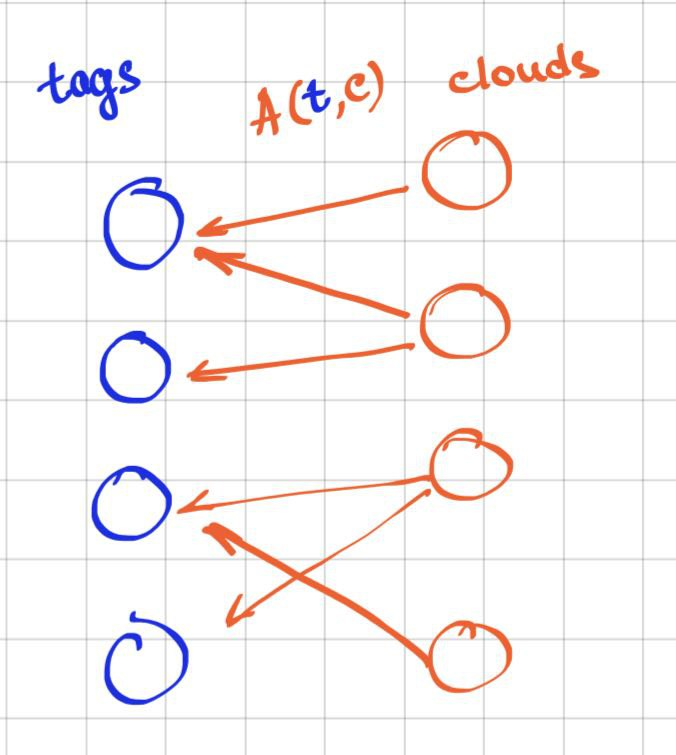
\includegraphics[scale=.25]{bipartite.jpg}
    \caption{The bipartite graph picture shows only edges with nonzero values.}
    \label{fig:nice_name}
\end{figure}

To be more specific, we are given a set of clouds $C = \{c_1, \dots, c_k\}$, and a set of tags $T = \{t_1, \dots, t_n\}$.
Each tag $t_i \in T$ and cloud $c_j \in C$ are related by the attention---the real value $a_{ij}$---that the cloud pays to the tag.
Let's agree that the greater the value, the higher the attention is. Naturally, the absence of attention corresponds to $a_{ij} = 0$. 

All the values $a_{ij}$ are stored in a matrix $\mathcal{A}$; its row $\mathcal{A}_{i:}$ corresponds to tag $t_i$, its column $\mathcal{A}_{:j}$ corresponds to cloud $c_j$.

This tag-cloud-attention metaphor applies to many problems in bioinformatics and statistics (see Tab.\ref{tab:examples} for examples).

\begin{table}[h!]
\centering
\begin{tabular}{c|c|c|c}
\textbf{Example} & \textbf{tag $t_i$} & \textbf{cloud $c_j$} & \textbf{attention $a_{ij}$} \\ 
\hline
\begin{tabular}[c]{@{}c@{}}gene regulation\\  by TFs\end{tabular}     & gene             & \begin{tabular}[c]{@{}c@{}}genes under \\ TF regulation\end{tabular}     & \begin{tabular}[c]{@{}c@{}}strength of \\ regulation\end{tabular}       \\ \hline
\begin{tabular}[c]{@{}c@{}}transcription \\ correlations\end{tabular} & gene             & \begin{tabular}[c]{@{}c@{}}genes coexpressed \\ with a gene\end{tabular} & \begin{tabular}[c]{@{}c@{}}transcription \\ correlation\end{tabular}    \\ \hline
fuzzy clustering                                                      & object           & cluster                                                                  & \begin{tabular}[c]{@{}c@{}}object weight \\ in cluster\end{tabular}     \\ \hline
\begin{tabular}[c]{@{}c@{}}transcription\\ decomposition\end{tabular} & transcript       & \begin{tabular}[c]{@{}c@{}}transcription \\ pattern\end{tabular}         & \begin{tabular}[c]{@{}c@{}}transcript's \\ load in pattern\end{tabular} \\ \hline

\begin{tabular}[c]{@{}c@{}}weighted graph\end{tabular} & vertex       & \begin{tabular}[c]{@{}c@{}} another vertex \end{tabular}         & \begin{tabular}[c]{@{}c@{}}weight of edge between\\ cloud and tag \end{tabular} \\ \hline
\end{tabular}

\caption{Tag-cloud metaphor deployment examples.}
\label{tab:examples}
\end{table}


% \paragraph{Goal} 

%There is a simple intuition of what it means to be a friend. A friend of Augustus cares about Augustus more than about other people. And, if we see Augustus, then we infer to see friends(s) of Augustus also. Let’s translate it into statistical language.
% We remember that a friend of Augustus cares about Augustus more than about other people.



% \textcolor{purple}{For each tag, we want to identify the cloud(s) that particularly prefer(s) the tag, if any. Then such a cloud is a friend (or the best friend if there is only one) for the tag. The simplest example: imagine that only one cloud pays attention to the tag in hand. }

Let's recall the intuition that starts the introduction. A friend of Augustus cares about Augustus more than other people do. 

We express how much a cloud $c_j$ cares about a tag $t_i$ in terms of the rank of $a_{ij}$ in column $\mathcal{A}_{:j}$. So, if a cloud $c_j$ cares about a tag $t_i$ more than other clouds, the rank of $a_{ij}$ in $\mathcal{A}_{:j}$ is higher than the rank of $a_{il}$ in $\mathcal{A}_{:l}$ for all $l \neq j$. 

A question naturally arises: whether $c_j$ is a real best friend of $t_i$ or $c_j$ appeared at the top of the ranking just because there is always something at the top.
 
\textcolor{blue}{We intend to statistically answer the question.}

Under $H_0$ we assume that all the clouds do not tell tags from each other.
In other words, all the $n \times k$ attention values from clouds to tags are independent (all $a_{ij}$ are independent). Moreover, all the $n$ attention values that a cloud pays to tags are identically distributed (all $a_{ij} \in \mathcal{A}_{:j}$ are i.i.d).

\textcolor{red}{Explain $H_1$! : The event "c is a friend of t" is a property of the entire $\mathcal{A}$ rather than of specific indices}

\textcolor{blue}{Here, we suggest a computational method...}

\textcolor{violet}{\begin{itemize}
    \item The {\cloud} is referred to as the {\tag}'s best friend and the test is named "the best friends test" or "the gene's best friends test".
    \item Marker
    \item Above, we consider only one possible best friend (cloud) per tag. The statistics naturally expand to the case when a {\tag} selects (separates) a subset of {\cloud}s, thus having more than one best friend.
\end{itemize}}


\section{Literature survey}
\textcolor{red}{literature survey ctd here}
\textcolor{purple}{We formulated \cite{best_friends:2015} the similar task in a symmetric form on gene expression data as searching for genes that are best friends of genes. Best friend of a gene $G_i$ is another gene $G_j$ that is expressed concertedly with the gene $G_i$, while other genes $G_k, k\neq i, k \neq j$ are (almost) not. The best friend is unique, while one gene can be the best friend for more than one gene. The solution we proposed (rank backwards ranking) showed the putative pairs of marker and its best friend, but it did not provide either statistical measure or an effect size estimate. Later, the problem was also formulated in an asymmetric setup \cite{patternmarkers:2017} for genes and expression patterns, and the solution was to scale each gene's loads to $max((\mbox{all loads for this gene})==1$ and calculate the Euclidean distance between the scaled vector of loads and the ideal $(0,0,...,1,...0$). The less the distance is, the better the marker is. }

\textcolor{blue}{+ Friedman test }
%\url{https://en.wikipedia.org/wiki/Friedman_test}

\textcolor{blue}{+ \cite{Gut:2009}}


%We formulated \cite{best_friends:2015} the similar task in a symmetric form on gene expression data as searching for genes that are best friends of genes. Best friend of a gene $G_i$ is another gene $G_j$ that is expressed concertedly with the gene $G_i$, while other genes $G_k, k\neq i, k \neq j$ are (almost) not. The best friend is unique, while one gene can be the best friend for more than one gene. The solution we proposed (rank backwards ranking) showed the putative pairs of marker and its best friend, but it did not provide either statistical measure or an effect size estimate. Later, the problem was also formulated in an asymmetric setup \cite{patternmarkers:2017} for genes and expression patterns, and the solution was to scale each gene's loads to $max((\mbox{all loads for this gene})==1$ and calculate the Euclidean distance between the scaled vector of loads and the ideal $(0,0,...,1,...0$). The less the distance is, the better the marker is. 

% Now, the question. For each tag, we want to identify the cloud(s) that specifically prefer(s) the tag. We say that such a cloud is a friend (or the best friend if it is the only one) for the tag. The simplest example: imagine that only one cloud pays attention to our tag. 


% 
%For a similar test that splits all the clouds into $m$ friends of the tag and the remaining $|C|-k$ clouds uses the difference  $r(t_i,c_{(m+1)}(t_i))$ and $r(t_i,c_{(m)}(t_i))$. If we obtain the p-value that is small enough, we claim that the clouds $c_{(1)}(t_i)$..$c_{(m)}(t_i)$ are friends of $t_i$ and $t_i$ is their marker.




%\section{Introduction: friends and markers}


% Let's picture a set of genes and their loads in expression patterns. Each pattern describes the expression of the genes in some process. Sometimes, we can conclude that a pattern is expressed from the expression of a single gene. The simplest case that allows this inference is when the gene has a nonzero load in only one pattern. The situation when other loads are just relatively small also fits the inference. We will refer to the gene as a marker gene and to the pattern as the best friend of the gene. Given the load matrix, we want to identify the marker genes and their best friends.


\section{Method}
\label{sec:method}


We recall that the attention matrix $\mathcal{A}$ is the only input for the statistical test. Each its element $a_{ij}$ is the value of attention that a cloud $c_j \in C$ pays to a tag $t_i \in T$
\[
\mathcal{A} = \begin{pmatrix}
a_{11} & a_{12} & \dots & a_{1k} \\
       &\cdots & \cdots &  \\
a_{n1} & a_{n2} & \dots & a_{nk}
\end{pmatrix}.
\]
Its $i$-th row corresponds to tag $t_i$, and we denote it as $\mathcal{A}_{i:} = (a_{i1}, \dots, a_{ik})$. Its $j$-th  corresponds to cloud $c_j$, and we denote it as $\mathcal{A}_{:j} =(a_{1j}, \dots a_{nj})'$ (with $'$ being transposition).

%from intro We express how much a cloud $c_j$ cares about a tag $t_i$ in terms of the rank of $a_{ij}$ in column $\mathcal{A}_{:j}$. So, if a cloud $c_j$ cares about a tag $t_i$ more than other clouds, the rank of $a_{ij}$ in $\mathcal{A}_{:j}$ is higher than the rank of $a_{il}$ in $\mathcal{A}_{:l}$ for all $l \neq j$. 

We do the following procedure to identify the cloud, which is the putative best friend (or, in other words, the most friendly cloud) for each tag.

For each cloud $c_j \in C$, we decreasingly rank the elements inside $\mathcal{A}_{:j}$. Thus, for each $a_{ij} \in \mathcal{A}_{:j}$, we get the ordinal number $r_{ij}:=\text{rank}\left(a_{ij}|\text{inside}~\mathcal{A}_{:j}\right)$. We resolve ties by the mean rank of the tied elements. 

Let's denote the rank matrix as 
\[
\mathcal{R} = \begin{pmatrix}
r_{11} & r_{12} & \dots & r_{1k} \\
       &\cdots & \cdots &  \\
r_{n1} & r_{n2} & \dots & r_{nk}
\end{pmatrix}, 
\quad
r_{ij} =\text{rank}\left(a_{ij}|\text{inside}~\mathcal{A}_{:j}\right).
\]
We denote its $i$-th row as $\mathcal{R}_{i:} = (r_{i1}, \dots, r_{ik})$.

To quantitatively express friendliness, we order the attention ranks to the same tag $t_i$ from different clouds. We decreasingly rank the elements in $\mathcal{R}_{i:}$ and the minimal element
corresponds to the cloud that is the putative best friend of $t_i$.

Let's denote the cloud-index (the second index) of the smallest entry in $\mathcal{R}_{i:}$ as $\sigma_i(1)$, the cloud-index of the second smallest entry as ${\sigma_i(2)}$, etc. The corresponding clouds are $c_{\sigma_{i}(1)}$, $c_{\sigma_{i}(2)}$, etc. 

So the putative best friend for the tag $t_i$ is the cloud $c_{\sigma_{i}(1)}$.

\subsection{The best friend test}
\label{sec:best_friend_test}

For a cloud to be a tag's best friend, it is \textit{necessary} to be the putative best friend, but it is \textit{not enough}. Indeed, in any ranking, there is the first element. We aim to statistically estimate whether the most friendly tag is the most friendly by chance. 

We recall that under $H_0$ all $a_{ij}$ are independent and all $a_{ij} \in \mathcal{A}_{:j}$ are i.i.d. So, by the construction, under $H_0$ all $r_{i\sigma(j)}$ are independent and uniformly distributed.

The smallest entry in $\mathcal{R}_{i:}$ is $r_{i\sigma_i(1)}$, the second smallest entry is $r_{i\sigma_i(2)}$, etc. For simplicity, we do not write the secondary $i$ index that is the same by construction as the first $i$. The resulting matrix is 
\[
\mathcal{R}_{\sigma} = \begin{pmatrix}
r_{1\sigma(1)} & r_{1\sigma(2)} & \dots & r_{1\sigma(k)} \\
       &\cdots & \cdots &  \\
r_{n\sigma(1)} & r_{n\sigma(2)} & \dots & r_{n\sigma(k)}.
\end{pmatrix}
\]

Under $H_0$, the entries of each $\mathcal{R}_{i:}$ are independently uniformly distributed. 

Thus, we can analytically estimate the distribution of the difference between the minimal and the next minimal values,
\[
U = \frac{r_{i\sigma(1)} - r_{i\sigma(2)}}{n}. 
\]
The $n$-normalization is technical. We explain it in more detail and we analytically obtain the distribution of $U$ under $H_0$ (denote it as $P(U ~|~ H_0)$) in Section \ref{sec:theory}. 

To test whether the putative best friend for the tag $t_i$ is really the best friend, we use the observed  (i.e. calculated for given $\mathcal{A}$) difference:
\[
u_1(t_i) = \frac{r_{i\sigma(1)} -  r_{i\sigma(2)}}{n}.
\] 

We estimate $p$-value for the pair of $t_i$ and its putative best friend $c_{\sigma_{i}(1)}$ using $u_1(t_i)$,
\[
p = P\left(U \ge u_1(t_i)~|~H_0\right). 
\]

If $p$-value is small enough, we reject the null and claim that the friendliness of the cloud $c_{\sigma_{i}(1)}$ is unlikely to observe by random, and so we refer to it as the best friend of $t_i$. In this case, $t_i$ is a \textcolor{red}{marker} of its best friend cloud $c_{\sigma_{i}(1)}$.

\subsection{The friends test}
\label{sec:friends_test}

In some cases, a tag has several clouds that are almost equally friendly to it. 
For example, a gene (tag) has a high load in two patterns (two clouds), and all other genes are low in both clouds. The tag (let it be $t_i$) is a marker for two clouds $c_{\sigma_{i}(1)}$ and $c_{\sigma_{i}(2)}$. However, the best friend statistics for $t_i$ cannot find either of the two. 
Indeed, $c_{\sigma_{i}(1)}$ is better than $c_{\sigma_{i}(2)}$ just by chance and $H_0$ is correctly not rejected by the best friend test.

Still, it is possible that there are two consecutive clouds $c_{\sigma_i(l)}$ and $c_{\sigma_i(l+1)}$, and the gap between these is statistically significant.

We denote the first $l$ clouds that are most friendly as $F_{i}(l) = \left\{ c_{\sigma_i(1)} \dots c_{\sigma_i(l)} \right\}$.
We aim to check whether $F_{i}(l)$ is really a set of friends of the tag $t_i$. Numerically, it means that the gap 
\[
u_{l}(t_i) = \frac{r_{i\sigma(l)} - r_{i\sigma(l+1)}}{n}
\]
is too large to be observed by chance if the null hypothesis $H_0$ holds. We note that $H_0$ is the same as in the \test{best friend test} (see Section \ref{sec:best_friend_test}).
Moreover, \test{best friend test} is a particular case of
this test---we will refer to it as \test{friends test}---with $l = 1$.

% In these cases, we extend the best friends test (see Section \ref{sec:best_friend_test}) to the friends test. 

 

% To possibly reject $H_0$ in these cases, we extend the best friends test (see Section \ref{sec:best_friend_test}) to the friends test. 





% The \test{friends test} possibly rejects $H_0$
% for the decomposition of $C$ into two group, $ F_{i}(l)$ and all the other clouds.

By analogy with \test{best friend test}, we asses $p$-value for $u_{l}(t_i)$
%for the pair of $t_i$ and the population $l$ of the subset of clouds $ \left\{ c_{\sigma_i(1)} \dots c_{\sigma_i(l)} \right\},$ that are putative friends between using $u_{l}(t_i)$,
\[
p = P\left(U \ge u_l(t_i)~|~H_0\right). 
\]
Again, we reject the null if the $p$-value is small enough. So, $F_{i}(l)$ are friends of $t_i$, and $t_i$ is their marker.


\subsection{Multiple tests, multimurkers}After the correction this p-value for multiple hypothesis testing (each feature provides its own null hypothesis), we identify the statistically significant pairs of a feature (marker) and entity (its best friend).

After the correction this p-value for multiple hypothesis testing (each feature provides its own null hypothesis), we identify the statistically significant pairs of a feature (marker) and entity (its best friend).


\subsection{The code availability}








%(they come from the same distribution).

%\subsection{Asymmetric $\mathcal{A}$}

%In case of asymmetric $\mathcal{A}$ the ...

%\subsection{Symmetric $\mathcal{A}$}
\section{Distribution under $H_0$: analytical form}
\label{sec:theory}
To get the analytical form for the $U$ distribution, we have to renormalize 
matrix $\mathcal{R}_{\sigma}$. Following the framework by \cite{Solomon2018OptimalTO}, we \textcolor{red}{...}

Let's denote
\[
\textcolor{red}{u_{ij}} = \frac{r_{i\sigma(j)} - \frac{1}{2}}{n}.
\]



% By construction, all the elements of $\mathcal{R}$ are uniformly distributed and independent.


\subsection{The best friend test}

% +\subsection{Multiple marker rank statistics}



%============
For each feature (tag!) $i,i=1\dots k$, we obtain a vector $r_{ij}, j=1..n$. There are normalised ranks of the feature in different entities, in the a null hypothesis they are uniformly i.i.d. in [0,1]. Let's create a rank statistics $u_i$ by ordering their values. If a feature is a unique marker for an entity, the entity corresponds to the first  value $u_1$. Let's use the difference $u_2-u_1$ as a measure of uniqueness (quality of the marker). Indeed, if we see that the difference is significantly higher than we can expect if null hypothesis holds, we can conclude that the feature unexpectedly prefer the entity, so it is a marker (and the entity is its best friend). Similarly to the density estimation for each $u_i$ (see, e.g. \cite{Gut:2009}) we estimate the probability to observe the difference $u_2 - u_1 \ge t$. 

First, the whole n-dimension (nD) volume of ranked variables $u_1 .. u_n$ is:
\begin{eqnarray*}
V = &\displaystyle \int_0^1\int_{u_1}^1\int_{u_2}^1\int_{u_3}^1...\int_{u_{n-1}}^1 du_n....du_4 du_3 du_2 du_1 =  \frac{1}{n!}
\end{eqnarray*}
see eq. \ref{eq:volume} for details.

Let's denote the p-value for the observation $t=u_2-u_1$ as $p_1(t)$. $p_1(t)$ is the ratio of the nD volume, that is limited by $t<=u_2-u_1$ condition, and $V$.

\begin{eqnarray*}
p(t) = & \displaystyle\frac{1}{V} \displaystyle \int_0^{1-t}\int_{{u_1}+t}^1\int_{u_2}^1\int_{u_3}^1...\int_{u_{n-1}}^1 du_n....du_4 du_3 du_2 du_1 = (1-t)^n
\end{eqnarray*}
see eq. \ref{eq:p_1} for details.

After the correction of this p-value for multiple hypothesis testing (each feature provides its own null hypothesis), we identify the statistically significant pairs of a feature (marker) and entity (its best friend).

\subsection{The friends test}
Now, let's suppose that a tag has more than one cloud, that almost equally good marks it, for example, two genes has nonzero load in a pattern. The pattern is the best friend for both of them, and each of them or their combination is a unique marker for the pattern, but the single marker rank statistics cannot find them, for the distance $u_2-u_1$ is quite low: the markers are almost equally good.

\section*{Notes and comments}

For a symmetric case, sometimes it makes sense to remove the main diagonal before ranking not to obtain trivial self-relations.

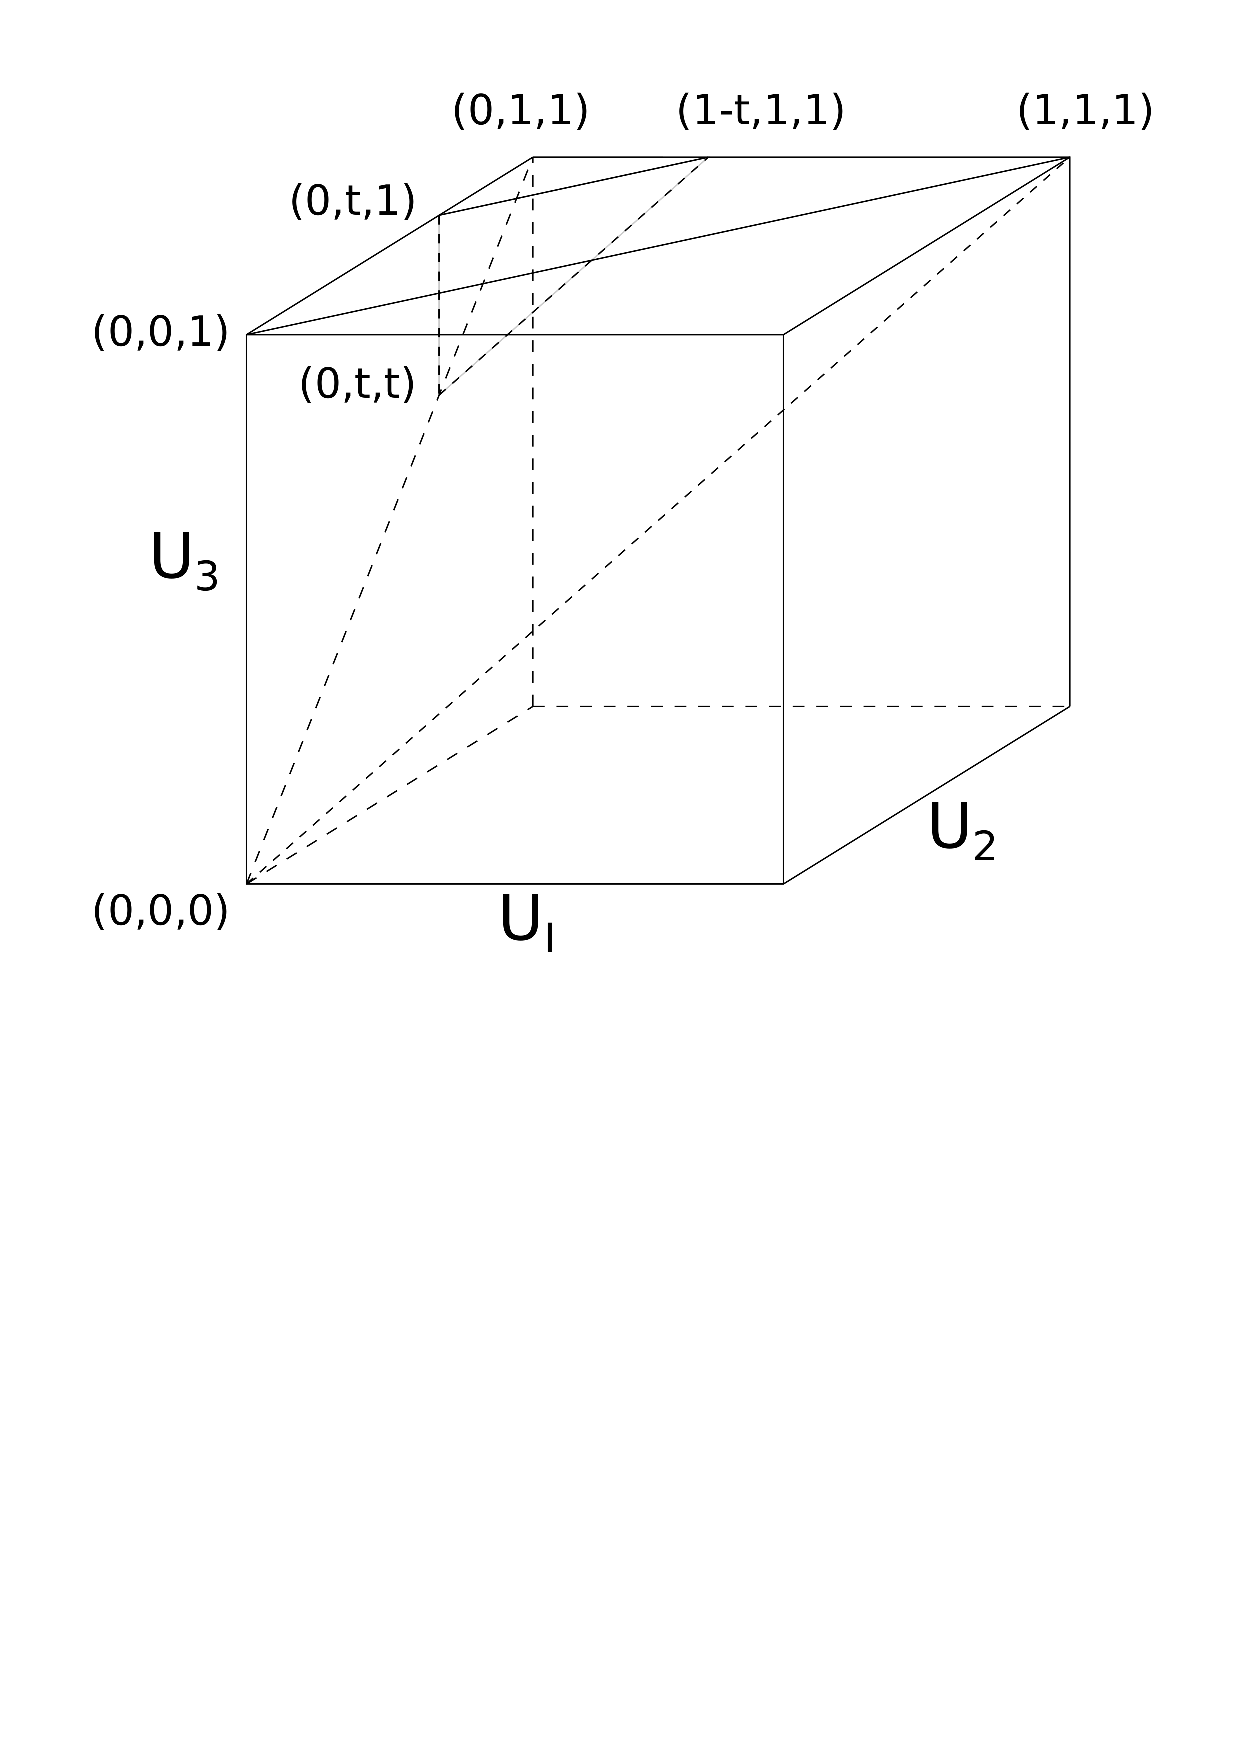
\includegraphics[scale=.5,trim=0 10cm 0 0, clip=true]{rank3d-nocolour}

The figure explains the probability estimation for the $n=3$ case. The rank statistics probability density is $3!=6$ and it uniformly scattered in (0,0,0), (0,0,1), (0,1,1), (1,1,1) tetrahedron. The $u_2 - u_1 \ge t$ condition holds only in the (0,t,t), (0,t,1), (0,1,1), (1-t,1,1) small tetrahedron.

To assess the p-value for a feature $i$, we do not need to rank the whole $r_{ij}, j=1..n$ vector to build the rank statistics $u_j$; we actually need only the $t$ value, so it is enough to find the maximal and the second values of $r_{ij}$.

\section{Discussion}

We formulated a statistical test that to detest reliable pairs of marker feature and the marked entity. Nevertheless the formulation of the problem looks abstract, its solution provides numerous straightforward application. The motivating example we started with was to detect the marker genes for expression patterns. The patterns could be obtained from the CoGAPS (scCoGAPS) \cite{Fertig_2016} or other matrix factorisation method \cite{Stein_2018}. The identification of the marker genes can critically simplify biological interpretation. If the matrix is the amplitude component from  the decomposition, the marker time points (or, the marker cells for scCoGAPS) can also be very informative for analysis. If the matrix contains the expression correlation for two gene sets, annotated best friends of an non-annotated gene extend the existing annotation.

\section{Conflict of interest}
The authors declare no conflict of interest.

\section{Acknowledgements}
AF acknowledges support by National Institutes of Health (NIH) P30CA006973 and 1U01CA253403-01, Russian Foundation for Basic Research (RFBR) 17-00-00208, the Russian Academy of Sciences Project 0112-2019-0001; VR acknowledges support from RFBR 20-54-12008; AM acknowledges support from RFBR 20-04-00459.

\bibliography{gene-best-friends}

\bibliographystyle{splncs03}
%\begin{subappendices}

\newcommand{\beginsupplement}{%
        \setcounter{table}{0}
        \renewcommand{\thetable}{S\arabic{table}}%
        \setcounter{figure}{0}
        \renewcommand{\thefigure}{S\arabic{figure}}
        \setcounter{equation}{0}
        \renewcommand{\theequation}{S\arabic{equation}}%
     }
\section*{Supplement}
\beginsupplement

%\renewcommand{\thesection}{\Alph{section}}%
% or try \arabic{section}
For an integer $m$,
\begin{eqnarray}
&\displaystyle \int_a^b\left(b-x\right)^{m-1}dx=
%-\displaystyle \int_0^{1-a}v^{n-1}dv=
\displaystyle \frac{\left(b-a\right)^m}{m}  \label{eq:intab}
\end{eqnarray} 
%\begin{eqnarray}
%&\displaystyle \int_a^1\left(1-x\right)^{m-1}dx=
%-\displaystyle \int_0^{1-a}v^{n-1}dv=
%\displaystyle \frac{\left(1-a\right)^m}{m}  \label{eq:right}
%\end{eqnarray} 
%\begin{eqnarray}
%&\displaystyle \int_0^b\left(b-x\right)^{m-1}dx=\displaystyle \frac{b^m}{m}  \label{eq:left}
%\end{eqnarray}
Applying \ref{eq:intab} recursively from $u_n$ until $u_1$: 
\begin{eqnarray}
V = &\displaystyle \int_0^1\int_{u_1}^1\int_{u_2}^1\int_{u_3}^1...\int_{u_{n-1}}^1 du_n...du_4 du_3 du_2 du_1 = \nonumber \\ 
&\displaystyle \frac{1}{(n-3)!}\int_0^1\int_{u_1}^1\int_{u_2}^1 \left( 1-u_3 \right)^{n-3}du_3 du_2 du_1 = \nonumber \\
&\displaystyle \frac{1}{(n-2)!}\int_0^{1-t}\int_{{u_1}+t}^1\left( 1-u_2 \right)^{n-2} du_2 du_1 = \nonumber \\
&\displaystyle \frac{1}{(n-1)!} \int_0^1\left( 1-u_1 \right)^{n-1} du_1 = \frac{1}{n!} \label{eq:volume}
\end{eqnarray} 
\begin{eqnarray}
& p_1(t) =  \displaystyle \frac{1}{V}\displaystyle \int_0^{1-t}\int_{{u_1}+t}^1\int_{u_2}^1\int_{u_3}^1...\int_{u_{n-1}}^1 du_n...du_2 du_1 =  \nonumber \\ 
%&\displaystyle \frac{n!}{(n-3)!}\int_0^{1-t}\int_{{u_1}+t}^1\int_{u_2}^1 \left( 1-u_3 \right)^{n-3}du_3 du_2 du_1 =  \nonumber \\
&\displaystyle \frac{n!}{(n-2)!}\int_0^{1-t}\int_{{u_1}+t}^1\left( 1-u_2 \right)^{n-2} du_2 du_1 =  \nonumber \\
&\displaystyle n \int_0^{1-t}\left( 1-t-u_1 \right)^{n-1} du_1 = (1-t)^n \label{eq:p_1}
\end{eqnarray}
\begin{eqnarray}
& p_k(t) = \displaystyle \frac{1}{V}\displaystyle \int_0^{1-t}\int_{{u_1}}^{1-t}...\int_{u_{k-1}}^{1-t}\int_{u_k+t}^1...\int_{u_{n-1}}^1 du_n... du_1 =  \nonumber \\ 
& \displaystyle \frac{n!}{(n-k-1)!}\displaystyle \int_0^{1-t}\int_{{u_1}}^{1-t}...\int_{u_{k-1}}^{1-t}\int_{u_k+t}^1 \left( 1-u_{k+1} \right)^{n-k-1} du_{k+1}...du_1 =  \nonumber \\
& \displaystyle \frac{n!}{(n-k)!}\displaystyle \int_0^{1-t}\int_{{u_1}}^{1-t}...\int_{u_{k-1}}^{1-t} \left( 1-t-u_{k} \right)^{n-k} du_k...du_1 =  \nonumber \\
& \displaystyle \frac{n!}{(n-k+1)!}\displaystyle \int_0^{1-t}\int_{{u_1}}^{1-t}...\int_{u_{k-2}}^{1-t} \left( 1-t-u_{k-1} \right)^{n-k+1} du_{k-1}...du_1 =  \nonumber \\
& \displaystyle n \int_0^{1-t}\left( 1-t-u_1 \right)^{n-1} du_1 = (1-t)^n \label{eq:p_k}
\end{eqnarray}
%\end{subappendices}
\begin{comment}
\subsection{ex-abstract}
Suppose we have set of {\tag}s $\T$ and a set of {\cloud}s $\C$ of this {\tag}s with some fuzzy membership, e.g. there is a numeric measure of how an {\tag} is represented in a {\cloud} $A(\tl,\cl)$ for each pair $(\tl,\cl):\tl \in \T, \cl \in \C$. The higher the $A(\tl,\cl)$ value is, the more the {\tag} $\tl$ is involved in the {\cloud} $\cl$. The absence of the {\tag} in the {\cloud} is shown by the value that is minimal for the {\cloud}.

An example that is easy to think about is: genes are {\tag}s and their groups under regulation by same transcription factors (TF’s) form {\cloud}s, and A shows the strength of the regulation. We look at a gene and we want to know whether a TF is its friend, i.e. whether the TF specifically prefers (regulates) the gene. The na\"ive idea is to look for a TF that the gene is the most sensitive for. Still, it’s possible that this TF is the strongest for the most of the genes. Sometimes, it is what we want to find, but now we want to answer other questions, namely, what TF is the most specific factor for the gene and is the specificity enough to say that is does not look like a random outcome?

Sometimes, the {\cloud}s are in in one-to-one relation with the {\tag}s, e.g. each {\cloud} is a set of {\tag}s, which are neighbours of {\tag} in some graph. For this example, A is a weighted adjacency matrix of this graph. The friendship terminology emerges naturally from this case. The friendship relation itself is asymmetric: a friend cares about Augustus, while Augustus does not.
\end{comment}
\end{document}


